\documentclass[12pt]{article}
\usepackage[alf]{abntex2cite}
\usepackage[utf8]{inputenc}
\usepackage[portuguese]{babel}
\usepackage{caption}
\usepackage{graphicx}
\usepackage{ragged2e}
\usepackage{indentfirst}
\usepackage{float}
\usepackage[left=3cm,top=3cm,right=2cm,bottom=2cm]{geometry}
\addto\captionsportuguese{
\renewcommand{\contentsname}
  {Sumário}
}
\begin{document}
\begin{titlepage}
    \begin{center}
        \Large
        \textbf{Faculdade de Economia, Administração, Contabilidade e Atuária da Universidade de São Paulo}
        
        \large
        \vspace{0.4cm}
        Departamento de Administração
             
        \vspace{4cm}
        \textbf{Eduardo de Passos}

        \vspace{4cm}
        \textbf{O impacto da guerra da Ucrânia na cadeia de valor mundial}

        \vspace{8cm}
        São Paulo\\
        2022\\
             
    \end{center}
\end{titlepage}
\begin{titlepage}
    \begin{center}
        \vspace{4cm}
        \large\textbf{Eduardo de Passos}
             
        
        \vspace{4cm}
        \large\textbf{O impacto da guerra da Ucrânia na cadeia de valor mundial}
    \end{center}

        \vspace{4cm}
        \hspace{7cm}
        \begin{minipage}{22em}
            Trabalho de conclusão de curso
            apresentado ao Departamento de
            Administração da Faculdade de Economia,
            Administração e Contabilidade da
            Universidade de São Paulo como requisito  para a
            obtenção do título de Bacharel 
            em Administração de Empresas\\
            \textbf{Orientador: Prof. Dr. Celso Cláudio de Hildebrand e Grisi}
        \end{minipage}
              
        \hspace{7cm}
    
    \vspace{8cm}
    \begin{center}
        São Paulo\\
        2022\\
    \end{center}
\end{titlepage}

\tableofcontents
\pagebreak

\listoftables
\pagebreak

\listoffigures
\pagebreak

\section{Introdução}
\subsection{Problema da Pesquisa}
Em 24 de fevereiro de 2022 a Rússia iniciou um ataque à Ucrânia com o intuito de anexar o país de volta a seu território, dado que sua saída ocorreu durante a quebra da União das Repúblicas Socialistas Soviéticas (URSS) em 1991. Com esforço, as tropas ucranianas retardam o avanço das tropas russas e o conflito vem se estendendo desde fevereiro 2022.

Segundo o jornal \cite{rootsWarNYT22} o ataque foi iniciado por Vladmir Vladimirovitch Putin, atual presidente da Rússia. O texto destaca as declarações do mandatário sobre a Ucrânia e como lamentava a perda desse território. Os ataques têm como foco tomar posse da capital ucraniana, Kiev, porém as tropas ucranianas ainda resistem às investidas russas. 

Nesse sentido, além de retomar o poder sobre uma importante nação vizinha, outro motivo por trás do ataque era a intenção da Ucrânia se juntar à Organização do Tratado do Atlântico Norte (OTAN), que, segundo o presidente russo, representava uma ameaça direta a Rússia \cite{natoNYT}. Conforme as regras da OTAN, quando um país-membro é atacado é dever dos demais países fornecerem apoio e proteção (NYT). Assim, caso a Ucrânia tivesse participação nessa organização a possível retaliação poderia desencadear um conflito ainda maior ou teria evitado que a Rússia tentasse reaver um território que pertencia a extinta URSS.

Tendo isso em vista, as ações da Rússia têm causado impactos de grande escala na esfera social e econômica da Ucrânia, além de gerar um movimento de refugiados por toda a Europa. A falta de trabalhadores e a ausência de segurança para operação da indústria têm afetado amplamente a produtividade do país. Segundo estimativa do World Bank (2022) é esperada uma queda de 45\% no PIB da Ucrânia caso o conflito se estenda por mais meses.

Por outro lado, pelo lado da Rússia as consequências se dão pelas sanções impostas pelas demais nações em forma de retaliação pela invasão a Ucrânia. Por isso, é previsto que o PIB da Rússia seja reduzido em 11 pontos percentuais no ano de 2022, segundo dados do World Bank. Essa queda é puxada pela drástica diminuição nos números de importação e exportação, aspectos que tiveram as sanções mais severas impostas.

As consequências das sanções na Rússia e o impacto da invasão na Ucrânia causam um distúrbio nas cadeias valores mundiais, devido à quebra de produtividade de um e o isolamento imposto ao outro. Nesse cenário, os demais países necessitam se adaptar a esses eventos e procurar novos agentes para suprir demandas que estão atualmente instáveis.

\subsection{Objetivo do TCC}
Considerando que a guerra é um fato recente e ainda não terminou o limite de contexto a ser utilizado é o primeiro semestre de 2022, os dados utilizados também seguiram essa regra.

O propósito dessa pesquisa é entender como o conflito entre a Rússia e Ucrânia vai afetar a cadeia de valor mundial. Através de dados históricos e de análises das relações desses países serão apresentados os principais produtos que esses países têm influência e como sua escassez irá afetar as demais nações.

Além de entender quais os principais produtos que esses países comercializam, o estudo irá mostrar quais países terão um impacto positivo com aumento de demandas não mais supridas pelos países em guerra, bem como entender quais produtos não tem um exportador capaz de atender as demandas atuais. 

Por fim,serão estudados estudados os impactos econômicos tanto nas nações em conflito quanto nos blocos econômicos e em países que mantinha com algum ou ambos os paísesm comércio com algum ou ambos os países. Entender esses impactos possibilitará demonstrar como as cadeias de valor tem unido economias nacionais trazendo uma facilidade na produção e desenvolvimento em detrimento de aumentar os riscos sistêmicos.

\subsection{Objetivo Secundário}
O trabalho se dedicará, de forma secundária, a abordar como os impactos na cadeia de valor mundial podem afetar o Brasil. As mudanças que ocorreram no mundo podem abrir oportunidade para o Brasil, visto que ele é um grande exportador de \emph{‘commodities’}. Entretanto, tais mudanças podem afetar negativamente com a perda de volume de exportação e a perda de matéria-prima importada.

Tais impactos serão mencionados ao decorrer do estudo dos principais impactos mundiais, ressaltando os pontos que podem afetar a economia nacional. As mudanças na cadeia de valor mundial afetam questões econômicas nacionais como inflação, produto interno bruto e a geração de empregos. 

Ainda, tAinda, ter compreensão dos possíveis efeitos no Brasil é uma forma também de demonstrar a dependência da nossa economia em relação a economia mundal. Com aprofun,damento, é possível entender a fragilidade da economia brafrenteià leira frente  crises internacionais.

\subsection{Estrutura do Trabalho}
Esse estudo é divido em seis capítulos, de forma que haja uma maior delimitação entre os diversos temas abordados pelo estudo, possibilitando uma melhor contextualização do problema, as causas, o desenrolar e os potenciais efeitos. 

Dessa forma, o primeiro capítulo se tratará da introdução, onde será dado um prévio contexto do conflito, bem como a apresentação do objetivo principal e secundário do estudo. Também é apresentado o período de tempo de informações a serem utilizadas, visto que o conflito ainda está em curso.

Posteriormente, no segundo capítulo será apresentada a revisão da literatura sobre a globalização, todo seu contexto histórico e o que causou tais mudanças no cenário global o, de forma a mostrar como o advento da globalização impactou a existência da cadeia global de valor. No mesmo capítulo, será apresentado o conceito de cadeias de valor e sua importância no mundo moderno.

O terceiro e quarto capítulos se debruçarão sobre os estudos dos dois países envolvidos no conflito, com o objetivo de entender o histórico comercial de cada um deles e em qual contexto estavam inseridos antes da guerra. Além de estudar cada país, serão apresentados seus principais parceiros comerciais. Por fim, serão expostos os principais desafios para a retomada do comércio internacional e como o cenário atual têm afetado o desenvolvimento econômico dos países envolvidos.

O quinto capítulo apresenta a metodologia utilizada para obter os dados, realizar o seu tratamento e as formas com que serão analisados e expostos ao logo da pesquisa. 
\pagebreak

\section{Revisão Bibliográfica – Parte I}

\subsection{Globalização}
A globalização é o “processo de unificação entre diversas culturas, populações e economias” \cite{globalization18}. O mundo tem passado por um processo de “encolhimento” no qual se facilitou ter acesso a produtos, serviços, entretenimento e informações de outros países. Keynes, no ano de 1920, já havia percebido tal efeito mencionando que alguém em Londres poderia pedir por telefone o seu chá e demais produtos oriundos de diversas partes do planeta, além disso investir em novas empresas e explorar novos produtos \cite{keynes1920}.

Dado isso, muito se discute sobre as ondas de globalização que ocorreram durante a história, como consenso se dividiam em duas ondas, a primeira se situando antes 1914 e a segunda se iniciando no pós-guerra em 1945 \cite{krugman15}. Em 2018, Thomas Palley trouxe a hipótese das três ondas de globalização, a primeira em consenso com a teoria anterior, termina no período pré-Primeira Guerra em 1914, a segunda foi reduzida para o período de 1945 até 1990 e, por fim, a terceira onda que, com o advento da internet, teria se iniciado em 1990 e está acontecendo até os dias atuais \cite{palley2018three}. 


\begin{figure}[h]
    \begin{center}
        \caption{Três ondas de globalização}
        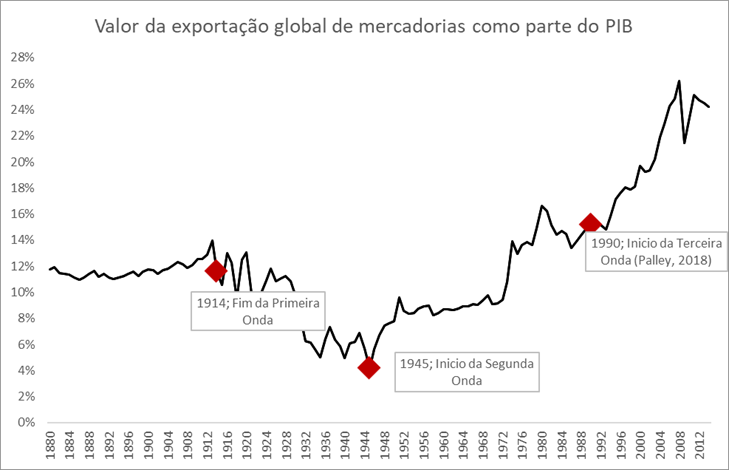
\includegraphics[width=0.8\textwidth]{globalização.png}
        \caption*{Fonte: Our world in data (2022), adaptado pelo autor.}
        \label{globalizacao}
    \end{center}
\end{figure}

De maneira específica, a primeira grande onda de globalização foi possível graças a evolução da tecnologia de comunicação, da infraestrutura e do transporte. Com o surgimento de telégrafo, das rodovias e das ferrovias, que favoreceram a evolução dos meios de locomoção e facilitaram a compra e venda de produtos, diminuiu-se o tempo necessário para obter os materiais para produção\cite{globalization18}. Além disso, a evolução das embarcações e sistemas de refrigeração foram pontos cruciais para o aumento do comércio entre a Europa - já industrializada e com alta eficiência de produção - e a América - em processo de expansão e desenvolvimento – o que trouxe uma evolução para a integração global do comércio \cite{palley2018three}. 

O fim da primeira onda veio com uma crise sem precedentes: a Grande Depressão (1929), que dizimou sistemas financeiros e economias ao redor do globo. Posteriormente, a Segunda Guerra Mundial se juntou aos fatores, ao extinguir grande parte do avanço realizado pela primeira onda de globalização. O autor James Harold explora no seu livro, “The End of Globalization”, os principais catalisadores para esse evento, como a fragilidade do sistema financeiro, o movimento antiglobalização com a imposição de restrições às importações favorecendo indústrias nacionais e a dificuldade em manter relações entre os países em períodos de guerra \cite{harold02}. 
Fazendo um paralelo com a situação atual entre a Rússia e Ucrânia, vemos sistemas financeiros fragilizados ainda se recuperando dos danos causados pela COVID-19 e políticas monetárias adotadas durante o período pandêmico mostrando os seus efeitos colaterais com os níveis de inflação se elevando constantemente. Nesse contexto, é possível prever que os impactos no comercio internacional serão de curto a médio prazo, em um cenário positivo (Banco Mundial, 2022).

Em 1945, marcado pelo fim da Segunda Guerra Mundial, teve início a segunda onda de globalização, amplamente explicada pela teoria de comercio intraindústria \cite{palley2018three}. Esse comércio trouxe a necessidade das indústrias se desenvolverem e terem uma evolução na produção, conceitos como ganho marginal e ganho de escala começaram a fazer parte das estratégias de grandes empresas que tinham de competir com o produto importado ou serem uma opção atrativa para exportação. A abertura comercial eleva a competição, fazendo com que o consumidor tenha uma variedade de escolhas a sua disposição, criando o cenário de competição perfeita, em que o mercado determina o preço e as indústrias procuram o reduzir os custos para aumentar as margens de ganho.

A terceira onda, proposta por Palley tem seu início no ano de 1990, tendo como principal conceito “cadeia de valor mundial”, aparecendo com mais ênfase junto às empresas multinacionais, que procuram diversificar a localização das fábricas e quais componentes são fabricados em cada parte do mundo, além de terceirizar parte da produção. A busca pela redução de custos trouxe como solução a especialização em produção de componentes e a procura pela melhor mão de obra, seja considerando o custo ou o conhecimento. Essa nova onda culminou em um conceito central para essa pesquisa que é a cadeia de valor global. 

\subsection{Cadeia de Valor Global}

Conforme a hipótese de Palley (2018), o mundo vive um momento de maior integração entre os países, no qual as empresas buscam a melhor alocação de sua produção definindo estrategicamente onde será mais vantajoso. 

Atualmente a produção pode ser dividida em quatro categorias \cite{wang2017measures}: produção doméstica, comércio tradicional, produção simples e produção complexa. Na primeira categoria, todo o processo produtivo do serviço ou do produto é feito no mesmo país, como exemplo temos um corte de cabelo. Na segunda, o produto é feito domesticamente, mas é vendido para outro país, como exemplo podemos citar um vinho português sendo vendido no Brasil. Por fim, as duas últimas categorias – fruto da produção por meio da cadeia de valor mundial – se caracterizam, respectivamente pela importação para produção uma única vez e pela diversidade de componentes e produtos importados de diversas partes do mundo, como exemplo a produção do iPhone ou de um automóvel.

A cadeia de valor complexa tem definido a globalização atualmente, na qual não existem mais fronteiras para as empresas e seus produtos e produção alcançam as mais diversas partes do mundo. Os benefícios já citados se caracterizam por obter o melhor produto ou serviço seja no custo ou qualidade, mas os riscos também aumentam devido à alta exposição a diversos fatores culturais e políticos. Ademais, a expansão global de produção e venda retira fronteiras domésticas de demanda fazendo com que o produto consiga chegar à onde existe a demanda, porém esse benefício vem com a necessidade de investimento em logística e se adaptar a padrões de preço e qualidade de diversos mercados \cite{riskOpportunities14}.
\pagebreak

\section{Revisão Bibliográfica – Parte II – Rússia}

\subsection{Principais Parceiros Comerciais}
Atualmente, grande parte do comércio russo é divido entre Europa, com 49,2\% das exportações, e a Ásia, com 42,3\% das exportações \cite{oecRussia22}. O principal parceiro econômico do país é a China, com quem têm estreitado alianças, principalmente depois da anexação da Criméia, ocasionando a perda de grande parte dos parceiros comerciais. Nesse sentido, os russos encontraram na China um aliado contra a dominância dos Estados Unidos e um grande cliente para a exportação de energia \cite{bloombergChinaRussia22}. 

Assim, o crescimento nas exportações chinesas é constante desde o episódio da Criméia, mas especificamente em 2021 o maior aumento foi com o Brasil, por meio do qual houve um aumento de 163,8\% das exportações \cite{workmanRussia22} sendo em maior parte fertilizantes e petróleo refinado \cite{oecRussia22}.

Entretanto, ponto negativo no comércio com a China é o déficit comercial, que é a diferença entre exportação e importação. A China apresenta o maior déficit comercial russo, com 4,6 bilhões de dólares de diferença. Outros grandes déficits são: Vietnam, França, Indonésia e Irlanda. \cite{oecRussia22}.

\subsection{Principais Produtos Exportados}

A Rússia tem 17,1 milhões de quilômetros quadrados, tornando-a o maior país em extensão territorial do mundo, isso traz uma vantagem no quesito recursos naturais e espaço para a agricultura. Em 2020 a Rússia foi a maior exportadora de trigo, ferro, peixe e níquel \cite{oecRussia22}, no quadro abaixo são apresentados os principais produtos exportados pela Rússia em 2020:

\begin{table}[H]
    \begin{center}
        \caption{Exportações Rússia 2020}
        \begin{tabular}{c}
            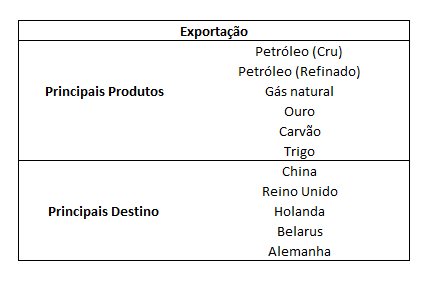
\includegraphics[width=0.6\textwidth]{exp rus.png}
        \end{tabular}
        \label{exprus}
        \caption*{Fonte: OEC (2022), adaptado pelo autor.}
    \end{center}
\end{table}

Dada a tabela, os principais produtos de exportação do país sofreram duras sansões dos Estados Unidos, que extinguiu qualquer comércio de petróleo ou gás com a Rússia; e da União Europeia que restringiu as importações de petróleo e planeja reduzir a de carvão também. O Reino Unido, segundo maior destino de exportações russa, tem também adotado sansões a importação de petróleo, e pretende zerar a importação caso o conflito não se encerre. Além disso, também está em discussão um embargo para qualquer importação de ouro russo \cite{russianGold22}, quarta maior exportação russa em 2020. É estimado que nos cem primeiros dias de guerra a Rússia tenha perdido US\$ 100 bilhões \cite{sanctionsRussiaBBC22}. 


\subsection{Principais Produtos Importados} 

A Rússia se destaca no mundo como o maior importador de óxido de alumínio, cobre, papel de parede e turbinas \cite{oecRussia22}. A tabela abaixo mostra os principais produtos importados pela Rússia no ano de 2020:

\begin{table}[H]
    \begin{center}
        \caption{Importações Rússia 2020}
        \begin{tabular}{c}
            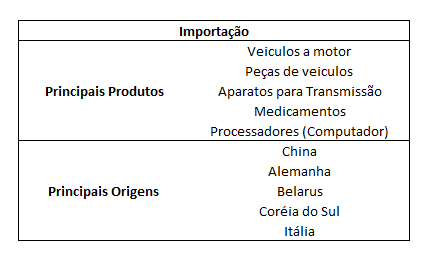
\includegraphics[width=0.6\textwidth]{imp rus.png}
        \end{tabular}
        \label{imprus}
        \caption*{Fonte: OEC (2022), adaptado pelo autor.}
    \end{center}
\end{table}

Os principais produtos importados pela Rússia são veículos a motor, que tem como principais fontes: Japão, Coréia do Sul, Alemanha, Estados Unidos e Eslováquia. Acompanhado dos veículos, a segunda maior importação são as peças para reparo ou montagem de veículos a motor, tendo como principal origem a Alemanha. Além dos carros a Alemanha é também a principal origem dos medicamentos importados no ano de 2020.

Ainda, a China, sua principal parceira comercial tanto em exportação quanto em importação, é responsável principalmente pela venda de aparelhos de transmissão e computadores que, em 2020, geraram US\$ 7 bilhões. No balanço total de 2020 a China exportou mais de cinquenta bilhões de dólares em produtos para a Rússia.

Assim, segundo a agência de notícias Bloomberg (2022), a saída das montadoras de carro da Rússia em retaliação a invasão na Ucrânia fez com que as vendas caíssem 79\% em abril. As montadoras que continuaram foram forçadas a interromper a produção devido à alta dependência das importações de peças.

\subsection{Principais Desafios}

O principal desafio comercial da Rússia é o crescente número de sansões aplicadas desde o início do conflito. Seus principais produtos têm sofrido sansões dos maiores compradores: a União Europeia e o Reino Unido. 

Outro ponto de atenção gasoduto russo, o “Nord Stream”, principal fonte de gás natural para grande parte de países europeus \cite{sanctionsRussiaBBC22}. Acredita-se que a compra deveria ser interrompida, mas a falta de um substituto impossibilita essa ação. 

Por fim, com a queda nas exportações e importações o desemprego também será um desafio, com a previsão de que 9\% dos russos estarão desempregados até o fim do ano \cite{russiaUnemployment22}. A falta de materiais para a produção e a queda no número de compradores são os principais motivadores para a debandada de empresas do país.

\pagebreak

\section{Revisão Bibliográfica – Parte III – Ucrânia}

\subsection{Principais Parceiros Comerciais}

A Ucrânia é um país com o poder comercial muito inferior ao da Rússia, em 2020 o país ficou nas colocações 46 e 47 em exportação e importação respectivamente, fechando o ano com déficit comercial, exportando US\$ 52 bilhões e importando US\$ 56 bilhões \cite{oecUkraine22}. 

Ademais, seus principais parceiros comerciais estão concentrados na Europa e na Ásia, sendo liderados pela China com um volume de US\$ 8 bilhões em exportações, que representa 12,1\% do total de exportações. Mesmo assim, o parceiro comercial que apresentou o maior crescimento em 2021 foi a Eslováquia com um aumento de 112\% das exportações.

\subsection{Principais Produtos Exportados}

A Ucrânia é a líder global na exportação de semente de girassol, sendo responsável por mais de 50\% da exportação global, principal componente na produção do óleo de cozinha. Além disso, também é referência na exportação de milho e trigo, produtos importantes na cadeia global de alimentos. A tabela a seguir mostra os principais produtos e parceiros de exportação:

\begin{table}[H]
    \begin{center}
        \caption{Exportações Ucrânia 2020}
        \begin{tabular}{c}
            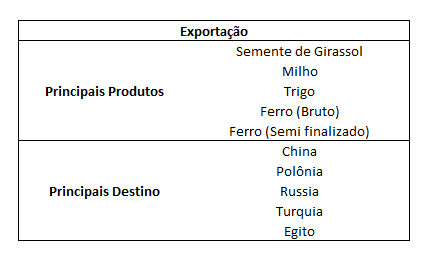
\includegraphics[width=0.8\textwidth]{exp ukr.png}
        \end{tabular}
        \label{impukr}
        \caption*{Fonte: OEC (2022), adaptado pelo autor.}
    \end{center}
\end{table}

Com efeito, a guerra causou um grande distúrbio no comércio de alimentos internacionais e a produção na Ucrânia tem sofrido com a invasão russa a seus principais portos e com o bloqueio naval no Mar Negro \cite{asiaFoodCrisis22} \cite{russianDevelopment22}. Enquanto agricultores não sabem como irão realizar a logística de entrega do seu produto aos clientes, países africanos, em especial, têm sofrido com o aumento dos preços \cite{asiaFoodCrisis22}. 

Nesse sentido, no dia 19 de maio de 2022 foi aprovado pelo Parlamento Europeu a suspensão de taxas de importação de produtos ucranianos, para gerar um maior suporte para a economia do país durante o período de guerra \cite{suspensionImports22}.

\subsection{Principais Produtos Importados}

Nas importações, a Ucrânia é a líder mundial na importação de lã, comprando US\$ 824 mil em 2020. A tabela a seguir apresenta os dados referentes a 2020:

\begin{table}[H]
    \begin{center}
        \caption{Importações Ucrânia}
        \begin{tabular}{c}
            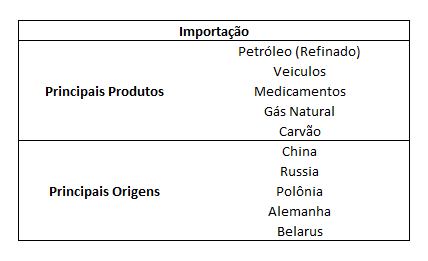
\includegraphics[width=0.8\textwidth]{imp ukr.png}
        \end{tabular}
        \caption*{Fonte: OEC (2022), adaptado pelo autor.}
        \label{expukr}
    \end{center}
\end{table}

Como observado, a importação de petróleo vem principalmente de Rússia e Belarus que, em conjunto, correspondem a mais de 70\% da importação de petróleo do ano de 2020. Os veículos importados são provenientes dos Estados Unidos, Japão, Polônia e Coréia do Sul. 

\subsection{Principais Desafios}

Com a perda de seus principais portos, e consequentemente o acesso ao Mar Negro, a distribuição do produto ucraniano é extremamente dificultada. Como consequência, vários países têm sofrido com a falta e com o aumento nos preços do trigo no primeiro semestre de 2022, principalmente países do norte africano, alcançando máximas históricas.
 
Tendo isso em vista, as medidas de isenção de tarifas nos produtos ucranianos é uma ótima medida que vai facilitar a venda dos produtos que ainda tem capacidade de ser produzidos, entretanto esse produto vai ser entregue na Europa, forçando os antigos importadores a procurarem outros exportadores. 
\pagebreak

\section{Metodologia de Pesquisa}

\subsection{Coleta de Dados}
A coleta de dados será realizada por meio dos dados disponibilizados nos sites especializados que ainda serão definidos. Ainda, dado que os fatos são recentes, nem todas as fontes de dados conseguirão cobrir o evento que ocorreu no primeiro semestre desse ano em sua totalidade. Demais informações sobre a previsão para a coleta dos dados se encontram no cronograma de entregas do TCC II.

\subsubsection{Coleta de dados de exportação}

Para a realização das análises de exportação serão utilizados os cinco principais produtos exportados no primeiro semestre de 2012 a 2022, divididos entre Ucrânia e Rússia, quantificados por mês com as variáveis: preço de venda em dólares, volume de venda em dólares e três principais compradores e o valor comprado. 

Desse modo, o preço de venda será utilizado para entender o momento do mercado, sendo um aumento da demanda gerando aumento do preço ou queda na demanda e baixa no preço. Em segundo lugar, o volume de vendas mostrará a capacidade dos países em produzir o produto e vendê-lo. Por fim, os três principais compradores e quantidade comprada serão importantes para compreender os impactos causados pela guerra, se houve uma diminuição do volume comprado e se houve alteração nos principais compradores.

\subsubsection{Coleta de dados de importação}

Para a realização das análises de importação serão utilizados os cinco principais produtos importados no primeiro semestre de 2012 a 2022, divididos entre Ucrânia e Rússia. Eles serão quantificados por mês com as variáveis: preço de compra em dólares, volume de compra em dólares, três principais vendedores e o valor comprado.

Assim, o preço de compra será utilizado para entender qual a situação do mercado. O volume de vendas auxiliará na compreensão da necessidade da Ucrânia pelo produto. E, por fim, os três principais vendedores indicarão posteriormente se essa demanda ficou represada ou se foi repassada para outro comprador.

\subsection{Métodos de Análise}

Para a análise dos dados será utilizado dois métodos: análise e regressão de dados. A análise exploratória do período anterior a guerra e outra no período posterior a guerra, tendo como foco entender as mudanças que ocorreram após o conflito, olhando o volume de vendas e compras e quais os produtos e países mais afetados.

Já na regressão de dados, serão utilizados dados do primeiro semestre de 2012 a 2022 para entender as mudanças causadas pela invasão no comportamento do mercado. Nesse intervalo, houve a crise causada pela pandemia de COVID-19, o qual também pode afetar nas estatísticas, mas será útil para observar qual foi o maior impacto no comércio. 

\subsubsection{Análise exploratória de dados}

Os dados semestrais de dez anos serão categorizados por mês para que fatores exógenos - como o clima - não sejam relevantes para produtos agrícolas. Assim, será explorada a média de preço e de vendas ou compras de cada produto escolhido por país, posteriormente, um boxplot do volume de vendas para encontrar outliers e ter uma análise visual dos números ao longo do tempo. É esperado que essas estatísticas mostrem como tem se comportado o comercio da Ucrânia e da Rússia na última década e que sejam mais perceptíveis as mudanças que ocorreram com a perda de poder produtivo ucraniano e os efeitos das sanções na Rússia.

A média aritmética é resultado da somatória de n valores, divididos pela quantidade de valor n, representada pela formula a seguir:
\[\overline{x} = \frac{x_1 + ... + x_n}{n} = \frac{1}{n}\sum_{i = 1}^{n}  x_i\]
	
Esse cálculo seráutilizado para estimar nto era esperado ser realizado seguindo a média dos anos anteriores e o quanto realmente foi realizado no ano de 2022. 
	
A seguir será feito um boxplot, com o objetivo de demonstrar mostrar a posição, dispersão, assimetria, caudas e dados discrepantes \cite{morettin2017estatistica}. Como mostra a imagem:

\begin{figure}[H]
    \begin{center}
        \caption{Boxplot}
        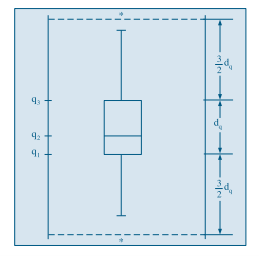
\includegraphics[width=0.6\textwidth]{boxplot.png}
        \caption*{Fonte: Morettin (2017)}
        \label{blxplot}
    \end{center}
\end{figure}

\subsubsection{Regressão linear simples}

A regressão linear simples tem como principal objetivo gerar uma equação que consiga explicar a correlação entre variáveis, dando assim uma previsibilidade para a média dos próximos valores. Tem o nome de linear pois é esperado que seja uma reta, como as variáveis escolhidas são preço, oferta e demanda é esperado que as correlações sejam lineares. A fórmula é mostrada a seguir:
\[E(Y|x) = \mu (x) = \alpha + \beta x\]

\pagebreak

\section{Cronograma de TCC II}

A seguir é apresentado o cronograma com todas as atividades a serem desempenhadas no segundo semestre de 2022. 

O cronograma se iniciará pela melhoria das partes já apresentadas adicionando referencias teóricas para um melhor embasamento e entendimento da situação. Além disso, a metodologia será expandida para melhor atender a quantidade e qualidade de dados.

Como os eventos são recentes, a disponibilidade de dados ainda é escassa. Assim, é esperado que no final de agosto já seja possível acessar os dados do primeiro semestre de 2022. Caso não seja possível a obtenção dos dados será refeita a metodologia de forma que se tenha a melhor quantificação dos impactos.

\begin{figure}[H]
    \begin{center}
        \caption{Cronograma TCC 2}
        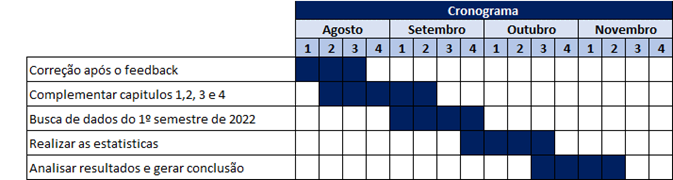
\includegraphics[width=0.8\textwidth]{cronograma tcc2.png}
        \label{crognograma}
    \end{center}
\end{figure}


\pagebreak
\bibliography{referencias}
\noindent{World Bank. 2022. "War in the Region" Europe and Central Asia Economic Uptade (Spring), Washington, DC: World Bank. Doi: 10.1596/978-1-4648-1866-0. License: Creative Commons Attribution CC BY 3.0 IGO}
\end{document}